\documentclass[12pt,space]{ctexart} %ans
\usepackage{GKExam}
\usepackage{tikz}
\usepackage{graphicx}
\usepackage{float}
\usepackage{caption}

\usetikzlibrary{positioning, shapes.geometric}
\begin{document}\zihao{5}
\juemi% 输出绝密
\biaoti{2017年普通高等学校招生全国统一考试(江苏卷)}
\fubiaoti{数学}
{\centering\heiti 注意事项 \\}
{\heiti 考生在答题前请认真阅读本注意事项及各题答题要求}
\begin{enumerate}[itemsep=-0.3em,topsep=0pt]
\item 本试卷共 \pageref{LastPage} 页,包含非选择题(第1题 - 第23题,共23题). 本卷满分为200分,考试时间为150分钟. 考试结束后,请将本试卷和答题卡一并交回. 
\item 答题前,请务必将自己的姓名、准考证号用0.5毫米黑色墨水的签字笔填写在试卷及答题卡的规定位置. 
\item 请认真核对监考员在答题上所粘贴的条形码上的姓名、准考证号与本人是否相符. 
\item 作答试题,必须用0.5毫米黑色墨水的签字笔在答题卡上的指定位置作答,在其他位置作答一律无效. 
\item 如需改动,须用2B铅笔绘、写清楚,线条、符号等须加黑、加粗. 
\end{enumerate}

\section{填空题:本大题共14小题,每小题5分,共计70分,请把答案填写在答题卡相应位置上}
\begin{enumerate}[itemsep=-0.3em,topsep=0pt]
  \item 已知集合$A=\{1,2\}$,$B=\{a,a^2+3\}$,若$A\bigcap B = \{1\}$则实数$a$的值为\blank{$1$}.
  \item 已知复数$z=(1+i)(1+2i)$,其中$i$是虚数单位,则$z$的模是\blank{$\sqrt{10}$}.
  \item 某工厂生产甲、乙、丙、丁四种不同型号的产品,产量分别为200,400,300,100件,为检验产品的质量,
        现用分层抽样的方法从以上所有的产品中抽取$60$件进行检验,则应从丙种型号的产品中抽取\blank{$18$}件.
  \item 图\ref{fig:a}是一个算法流程图,若输入$x$的值为$\displaystyle{\frac{1}{16}}$,则输出的$y$的值是\blank{$-2$}.
  \item 若$\displaystyle{\tan(\alpha-\frac{\pi}{4})=\frac{1}{6}}$,则$\tan\alpha=$\blank{$\frac{7}{5}$}.
  \item 如图\ref{fig:b},在圆柱$O_1O_2$内有一个球$O$,该球与圆柱的上、下面及母线均相切. 记圆柱$O_1O_2$的体积为$V_1$,
        球$O$的体积为$V_2$,则$\displaystyle{\frac{V_1}{V_2}}$的值是\blank{$\frac{3}{2}$}.
  
  \begin{figure}[H]
    \begin{minipage}[b]{0.45\textwidth}
      \centering
      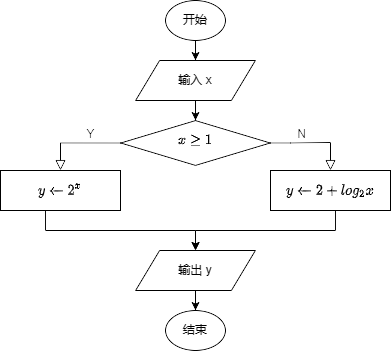
\includegraphics[width=1\textwidth]{Image/js-4.png}
      \caption{第 4 题}\label{fig:a}
    \end{minipage}
    \begin{minipage}[b]{0.25\textwidth}
      \centering
      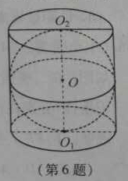
\includegraphics[width=0.9\textwidth]{Image/js-6.png}
      \caption{第 6 题}\label{fig:b}
    \end{minipage}
    \begin{minipage}[b]{0.25\textwidth}
      \centering
      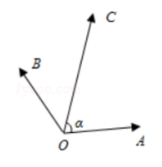
\includegraphics[width=1\textwidth]{Image/js-12.png}
      \caption{第 12 题}\label{fig:t12}
    \end{minipage}
  \end{figure}

  \item 记函数$\displaystyle{f(x)=\sqrt{6+x-x^2}}$的定义域为$D$. 在区间$[-4,5]$上随机取一个数$x$,
        则$x\in D$的概率是\blank{$\frac{5}{9}$}.
  \item 在平面直角坐标系$xOy$中,双曲线$\displaystyle{\frac{x^2}{3}-y^2=1}$的右准线与它的两条渐近线分别交于点$P$,$Q$,
        其焦点是$F_1$,$F_2$,则四边形$F_1PF_2Q$的面积是\blank{$4\sqrt{2}$}.
  \item 等比数列$\{a_n\}$的各项均为实数,其前$n$项的和为$S_n$,已知$\displaystyle{S_3=\frac{7}{4}}$,
        $\displaystyle{S_6=\frac{63}{4}}$,则$a_3=$\blank{$1$}.
  \item 某公司一年购买某种货物$600$吨,每次购买$x$吨,运费为$6$万元/次,一年的总存储费用为$4x$万元,要使一年的总运费与总存储之和最小,
        则$x$的值是\blank{$30$}.
  \item 已知函数$\displaystyle{f(x)=x^3-2x+e^x-\frac{1}{e^x}}$,其中$e$是自然数对数的底数,若$f(a-1)+f(2a^2)\leq 0$,
        则实数a的取值范围是\blank{$[-1, \frac{1}{2}]$}.
  \item 如图\ref{fig:t12},在同一个平面内,向量$\overrightarrow{OA}$,$\overrightarrow{OB}$,$\overrightarrow{OC}$的模分别为1,
        1,$\sqrt{2}$,$\overrightarrow{OA}$与$\overrightarrow{OC}$的夹角为$\alpha$,且$\tan\alpha=7$,$\overrightarrow{OB}$与
        $\overrightarrow{OC}$的夹角为$45^\circ$. 若$\overrightarrow{OC}=m\overrightarrow{OA}+n\overrightarrow{OB}$ $(m, n \in R)$,
        则$m+n=$\blank{$3$}.
  \item 在平面直角坐标系$xOy$中,$A(-12,0)$,$B(0,6)$,点$P$在圆$O: x^2+y^2=50$上,若$\overrightarrow{PA}\cdot\overrightarrow{PB}\leq 20$,
        则点$P$的横坐标的取值范围是\blank{$[-5\sqrt{2}, 1]$}.
  \item 设$f(x)$是定义在$R$且周期为$1$的函数,在区间$[0,1)$上,$\displaystyle{f(x)=\begin{cases}x^2,&x\in D\\x,&x\notin D\end{cases}}$
        其中集合$\displaystyle{D=\{x|x=\frac{n-1}{n}, n\in N_+\}}$,则方程$f(x)-\lg x=0$的解的个数是\blank{$8$}.
\end{enumerate}

\section{解答题:本大题共6小题,共计90分,请把答案填写在答题卡相应位置上}
\begin{enumerate}[itemsep=-0.3em,topsep=0pt,resume]
  \item (本小题满分14分)\\[0.5em] 
    \begin{minipage}[h][20ex][t]{.63\textwidth}
      如图\ref{fig:t15},在三棱锥$A-BCD$中,$AB\bot AD$,$BC\bot BD$,平面$ABD\bot$平面$BCD$,点$E$、$F$($E$与$A$、$D$不重合)分别在棱$AD$,$BD$上,
      且$EF\bot AD$. 求证:
      \begin{enumerate}[itemsep=-0.3em,label={(\arabic*)},topsep=0pt,labelsep=.5em,leftmargin=1.7em]
        \item $EF\parallel$平面$ABC$;
        \item $AD\bot AC$.
      \end{enumerate}
    \end{minipage}
    \begin{minipage}[h][20ex][b]{.35\textwidth}
      \begin{figure}[H]
        \centering
        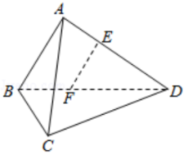
\includegraphics[width=0.6\textwidth]{Image/js-15.png}
        \caption{第 15 题}\label{fig:t15}
      \end{figure}
    \end{minipage}

  \item (本小题满分14分)\\
    已知向量$\boldsymbol{a}=(\cos x, \sin x)$,$\boldsymbol{b}=(3,\sqrt{3})$,$x\in [0,\pi]$。
    \begin{enumerate}[itemsep=-0.3em,label={(\arabic*)},topsep=0pt,labelsep=.5em,leftmargin=1.7em]
      \item 若$\boldsymbol{a}\parallel\boldsymbol{b}$,求$x$的值;
      \item 记$f(x)=\boldsymbol{a}\cdot\boldsymbol{b}$,求$f(x)$的最大值和最小值以及对应的$x$的值.
    \end{enumerate}
  \quad

  \item (本小题满分14分)\\ 
    \begin{minipage}[h][26ex][t]{.65\textwidth}
      如图\ref{fig:t17},在平面直角坐标系$xOy$中,椭圆$E: \displaystyle{\frac{x^2}{a^2}+\frac{y^2}{b^2}=1}$ $(a>b>0)$的左、右焦点分别为$F_1$,$F_2$,
      离心率为$\displaystyle{\frac{1}{2}}$,两准线之间的距离为$8$. 点$P$在椭圆$E$上,且位于第一象限,过点$F_1$作直线$PF_1$的垂线$l_1$,
      过点$F_2$作直线$PF_2$的垂线$l_2$.
      \begin{enumerate}[itemsep=-0.3em,label={(\arabic*)},topsep=0pt,labelsep=.5em,leftmargin=1.7em]
        \item 求椭圆$E$的标准方程;
        \item 若直线$l_1$,$l_2$的交点$Q$在椭圆$E$上,求点$P$的坐标. 
      \end{enumerate}
    \end{minipage}
    \begin{minipage}[h][26ex][b]{.32\textwidth}
      \begin{figure}[H]
        \centering
        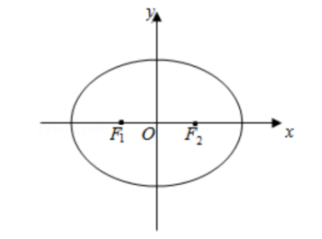
\includegraphics[width=1\textwidth]{Image/js-17.png}
        \caption{第 17 题}\label{fig:t17}
      \end{figure}
    \end{minipage}
  
  \begin{figure}[H]
    \centering
    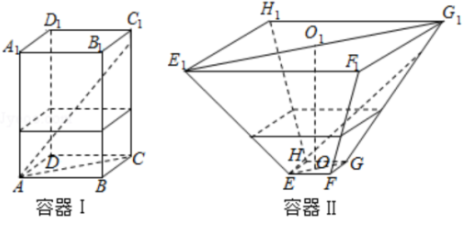
\includegraphics[width=0.5\textwidth]{Image/js-18.png}
    \caption{第 18 题}\label{fig:t18}
  \end{figure}
  \item (本小题满分16分)\\
    如图\ref{fig:t18},水平放置的正四棱柱形玻璃容器$I$和正四棱台形玻璃容器$II$的高均为$32cm$,容器$I$的底面对角线$AC$的长为$10cm$,容器$II$的两底面对角线$EG$,
    $E_1G_1$的长分别为$14cm$和$62cm$. 分别在容器$I$和容器$II$中注入水,水深均为$12cm$. 现有一根玻璃棒$l$,其长度为$40cm$.(容器厚度、玻璃棒粗细均忽略不计)
    \begin{enumerate}[itemsep=-0.3em,label={(\arabic*)},topsep=0pt,labelsep=.5em,leftmargin=1.7em]
      \item 将$l$放在容器$I$中,$l$的一端置于点$A$处,另一端置于侧棱$CC_1$上,求$l$没入水中部分的长度;
      \item 将$l$放在容器$II$中,$l$的一端置于点$E$处,另一端置于侧棱$CG_1$上,求$l$没入水中部分的长度.
    \end{enumerate}
    
  \item (本小题满分16分)\\
    对于给定的正整数$k$,若数列$\{a_n\}$满足$\displaystyle{a_{n-k}+a_{n-k+1}+\cdots+a_{n-1}+a_{n}+\cdots+a_{n+k-1}+a_{n+k}=2ka_n}$对任意正整数$n$ $(n>k)$总成立,
    则称数列$\{a_n\}$ 是“$P(k)$数列”.
    \begin{enumerate}[itemsep=-0.3em,label={(\arabic*)},topsep=0pt,labelsep=.5em,leftmargin=1.7em]
      \item 证明:等差数列$\{a_n\}$是“$P(3)$数列”;
      \item 若数列$\{a_n\}$既是“$P(2)$数列”,又是“$P(3)$数列”,证明:$\{a_n\}$是等差数列.
    \end{enumerate}
  
  \item (本小题满分16分)\\
    已知函数$f(x)=x^3+ax^2+bx+1(a>0,b\in R)$有极值,且导函数$f'(x)$的极值点是$f(x)$的零点。(极值点是指函数取极值时对应的自变量的值)
    \begin{enumerate}[itemsep=-0.3em,label={(\arabic*)},topsep=0pt,labelsep=.5em,leftmargin=1.7em]
      \item 求$b$关于$a$的函数关系式,并写出定义域;
      \item 证明:$b^2>3a$;
      \item 若$f(x)$,$f'(x)$这两个函数的所有极值之和不小于$\displaystyle{-\frac{7}{2}}$,求$a$的取值范围.
    \end{enumerate}
\end{enumerate}

\section{附加题:本大题共3小题,共计40分,请把答案填写在答题卡相应位置上}
\begin{enumerate}[itemsep=-0.3em,topsep=0pt,resume]
  \item 【选做题】本题包括A、B、C、D四小题,请选定其中两小题,并在相应的答题区域内作答。若多做,则按作答的前两小题评分。解答时应写出文字说明、证明过程或演算步骤。
  \begin{enumerate}[itemsep=-0.3em,label={\Alph*.},topsep=0pt,labelsep=.5em,leftmargin=1.7em]
    \item 【选修4-1:几何证明选讲】(本小题满分10分)\\[0.5em] 
      \begin{minipage}[h][20ex][t]{.65\textwidth}
        如图\ref{fig:t21A},$AB$为半圆$O$的直径,直线$PC$切半圆$O$于点$C$,$AP\bot PC$,$P$为垂足。求证:
        \begin{enumerate}[itemsep=-0.3em,label={(\arabic*)},topsep=0pt,labelsep=.5em,leftmargin=1.7em]
          \item $\angle PAC=\angle CAB$;
          \item $AC^2=AP\cdot AB$. 
        \end{enumerate}
      \end{minipage}
      \begin{minipage}[h][20ex][b]{.32\textwidth}
        \begin{figure}[H]
          \centering
          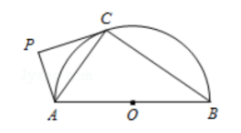
\includegraphics[width=0.9\textwidth]{Image/js-21-A.png}
          \caption{第 21 A 题}\label{fig:t21A}
        \end{figure}
      \end{minipage}
    
    \item 【选修4-2:矩阵与变换】(本小题满分10分)\\[0.4em] 
      已知矩阵$\displaystyle{A=\begin{bmatrix} 0 & 1 \\ 1 & 0 \end{bmatrix}}$,$\displaystyle{B=\begin{bmatrix} 1 & 0 \\ 0 & 2 \end{bmatrix}}$.
      \begin{enumerate}[itemsep=-0.3em,label={(\arabic*)},topsep=0pt,labelsep=.5em,leftmargin=1.7em]
        \item 求$AB$;
        \item 若曲线$\displaystyle{C_1: \frac{x^2}{8}+\frac{y^2}{2}=1}$在矩阵$AB$对应的变换作用下得到另一曲线$C_2$,求$C_2$的方程.
      \end{enumerate}
    \vspace{1ex}
    
    \item 【选修4-4:坐标系与参数方程】(本小题满分10分)\\
      在平面坐标系中$xOy$中,已知直线$l$的参考方程为$\displaystyle{\begin{cases}x=-8+t, \\ y = \displaystyle{\frac{t}{2}}\end{cases}}$($t$为参数),
      曲线$C$的参数方程为$\displaystyle{\begin{cases}x=2x^2, \\ y = 2\sqrt{2s}\end{cases}}$($s$为参数). 设$P$为曲线$C$上的动点,
      求点$P$到直线$l$的距离的最小值.
    \vspace{1ex}
    
    \item 【选修4-5:不等式选讲】(本小题满分10分)\\
      已知$a$,$b$,$c$,$d$为实数,且$a^2+b^2=4$,$c^2+d^2=16$,证明$ac+bd\leq 8$.
  \end{enumerate}

  \item (本小题满分10分)\\[0.5em]
    \begin{minipage}[h][20ex][t]{.63\textwidth}
      如图\ref{fig:t22},在平行六面体$ABCD-A_1B_1C_1D_1$中,$AA_1\bot $平面$ABCD$,且$AB=AD=2$,$AA_1=\sqrt{3}$,$\angle BAD=120^{\circ}$.
      \begin{enumerate}[itemsep=-0.3em,label={(\arabic*)},topsep=0pt,labelsep=.5em,leftmargin=1.7em]
        \item 求异面直线$A_1B$与$AC_1$所成角的余弦值;
        \item 求二面角$B-A_1D-A$的正弦值.
      \end{enumerate}
    \end{minipage}
    \begin{minipage}[h][20ex][b]{.35\textwidth}
      \begin{figure}[H]
        \centering
        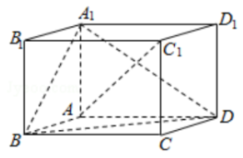
\includegraphics[width=0.6\textwidth]{Image/js-22.png}
        \caption{第 22 题}\label{fig:t22}
      \end{figure}
    \end{minipage}

  \item (本小题满分10)\\
    已知一个口袋有$m$个白球,$n$个黑球$(m,n\in N^*, n\geq 2)$,这些球除颜色外全部相同.现将口袋中的球随机的逐个取出,并放入如图所示的编号为1,2,3,$\cdots$,
    $m+n$的抽屉内,其中第$k$次取球放入编号为$k$的抽屉$(k=$1,2,3,$\cdots$,$m+n)$.\\
    \setlength{\tabcolsep}{7mm}{\begin{tabular}{|c|c|c|c|c|} 
      \hline 
      1&2&3&$\cdots$&$m+n$\\
      \hline  
    \end{tabular}}
    \begin{enumerate}[itemsep=-0.3em,label={(\arabic*)},topsep=0pt,labelsep=.5em,leftmargin=1.7em]
      \item 试求编号为2的抽屉内放的是黑球的概率$p$;
      \item 随机变量$X$表示最后一个取出的黑球所在抽屉编号的倒数,$E(X)$是$X$的数学期望\\
      证明:$\displaystyle{E(X)<\frac{n}{(m+n)(n-1)}}$.
    \end{enumerate}

\end{enumerate}

%%%%%%%%%%%%%%%%%%%%%%%%%%%%%%%%%%%%%%%%%%%%%%%%%%%%%%%%%%%%%%%%%%%%%%%%%%
%---------------------------------结束------------------------------------
%%%%%%%%%%%%%%%%%%%%%%%%%%%%%%%%%%%%%%%%%%%%%%%%%%%%%%%%%%%%%%%%%%%%%%%%%%
\clearpage

\end{document}
